\section{Metodologia}
\color{black}

A metodologia seguiu um fluxo evolutivo estruturado para transitar de capacidade computacional ilimitada
(Cloud) às restrições severas do Edge Computing, preservando performance competitiva.

\subsection{Cenários Operacionais}

\begin{itemize}
    \item \textbf{Cenário~1 --- Cloud:} Motor de treinamento principal, sem restrições de hardware.
    Permite modelos pesados de Deep Learning e processamento em lote de janelas longas~\cite{Le2025,
    Zhang2026}.
    \item \textbf{Cenário~2 --- Fog/Telemetria:} Dispositivo de borda atua como extrator de matrizes
    de características IoT. Transmissão via gRPC/MQTT reduz largura de banda evitando tráfego de
    áudio bruto~\cite{Uzel2026}.
    \item \textbf{Cenário~3 --- Edge/TinyML:} Inferência local no microcontrolador da máquina.
    Exige modelos compactados com latência $<50$~ms e memória $<4$~MB, com alertas autônomos ao
    sistema Web~\cite{Khamaisi2025}.
\end{itemize}

\subsection{Dados e Protocolo de Validação}

Quatro fontes de dados foram utilizadas, descritas na Tabela~\ref{tab:fontes_dados}.

\begin{table}[H]
\centering
\footnotesize
\begin{tabularx}{\columnwidth}{@{} l X X @{}}
\toprule
\textbf{Fonte} & \textbf{Tipo} & \textbf{Características} \\ \midrule
DCASE~2025 Task~2 & Pública & Sons industriais; First-Shot; Domain Shift~\cite{Nishida2025} \\
MIMII~DG & Pública & Fan, Pump, Slider, Valve; SNR: $-6$, 0, $+6$~dB~\cite{Dohi2022} \\
Kaggle Bearings & Pública & Rolamentos com falhas mecânicas reais \\
Drive Próprio & Privada & Áudios por celular; ambiente ruidoso real \\ \bottomrule
\end{tabularx}
\caption{Fontes de dados utilizadas no estudo.}
\label{tab:fontes_dados}
\end{table}

\textbf{Protocolo LOSO (\textit{Leave-One-Source-Out}):} Em cada rodada, uma fonte é mantida
exclusivamente para teste; as demais compõem treino/validação. O score final é a média das 4~rodadas.
Este protocolo elimina vazamento de dados entre fontes (anti-leakage) e mede generalização cross-domain
real, alinhando-se aos requisitos do DCASE~2025~\cite{Harada2023}.

\subsection{Cronologia Experimental: 4 Fases e 28 Experimentos}

O desenvolvimento seguiu roteiro incremental com técnicas descartadas documentadas a cada etapa,
conforme a Tabela~\ref{tab:cronologia_frentes}.

\begin{table}[H]
\centering
\footnotesize
\begin{tabularx}{\columnwidth}{@{} l X X @{}}
\toprule
\textbf{Etapa} & \textbf{Acréscimo Principal} & \textbf{Efeito no Sistema} \\ \midrule
Versão~1 & Janelas deslizantes + RPCA & Isolamento de transientes impulsivos \\
Versão~2 & HHT + Mel/MFCC/CWT & Enriquecimento espectral e estatístico \\
Versão~3 & NMF + Canal Híbrido & Erro de reconstrução como feature \\ \midrule
Frente~1 & L2 + Limiar Gamma & Menor sobreajuste e decisão estável \\
Frente~2 & CNN + GMM & GMM eleito campeão não supervisionado \\
Frente~3 & HHT+UKF completo & Limpeza e isolamento de transientes \\
Frente~4 & Mixup ($\alpha{=}0{,}4$) & Robustez ao domain shift \\
Frente~5 & pAUC@0.1 + Score DCASE & Foco em baixo falso alarme \\
Frente~6 & Gamma + FPR alvo & Limiar estatisticamente fundado \\
Frente~7 & Separação Protocolo A/B + DCASE~2025 & Comparação justa; alinhamento externo \\
Frente~8 & Arena não supervisionada & GMM confirmado; IF descartado \\
Frente~9 & Tiny-AST como gerador XAI & Deep Learning alocado a função auxiliar \\
Frente~10 & XAI visual completo & Diagnóstico temporal e espectral \\
Frente~11 & Consolidação multicritério & Protocolo LOSO completo \\ \bottomrule
\end{tabularx}
\caption{Cronologia das versões e frentes de melhoria do pipeline.}
\label{tab:cronologia_frentes}
\end{table}

\textbf{Fase~1 --- Exploração (NB~1--10):} Estabeleceu as bases por experimentação sistemática.
XGBoost emergiu campeão supervisionado (pAUC~0,97; 12~ms; $<$1~MB). GMM com $k{=}5$ componentes
adotado como campeão não supervisionado. Mel-Spectrogram eleito representação principal por integração
natural com MFCC e NMF. Teste cego revelou colapso inicial (pAUC: 0,9482 $\to$ 0,1111 por domain
shift), motivando as 11~Frentes de Melhoria.

\textbf{Fase~2 --- Otimização (NB~11--15):} HHT+UKF tornou-se primeiro estágio obrigatório. Mixup
melhorou pAUC cross-domain de 0,51 para 0,68 ($+33{,}3\%$). Adoção de pAUC@FPR~0.1 alterou ranking:
Tiny-AST caiu de 1º (F1=0,97) para 3º (pAUC=0,91); XGBoost+HHT ascendeu ao 1º lugar (pAUC=0,94).

\textbf{Fase~3 --- Validação (NB~16--21):} Limiar Gamma validado pelo teste Kolmogorov-Smirnov.
Outlier Exposure melhorou pAUC cross-domain para 0,76. Arena não supervisionada confirmou GMM;
Isolation Forest reprovado (pAUC~0,71). Tiny-AST definitivamente alocado ao XAI offline.

\textbf{Fase~4 --- Confrontamento (NB~22--28):} Ablation study revelou HHT+UKF como componente mais
crítico ($-7$~p.p.). Limite operacional formal documentado: Protocolo~B falha com SNR~$<-3$~dB sem
rótulos (MIMII Slider, SNR~$-6$~dB, pAUC~0,79~$<$~0,80).

\subsection{Arquitetura Final: Pipeline DIAMOND CRISTAL CLEAN}

\begin{figure}[H]
    \centering
    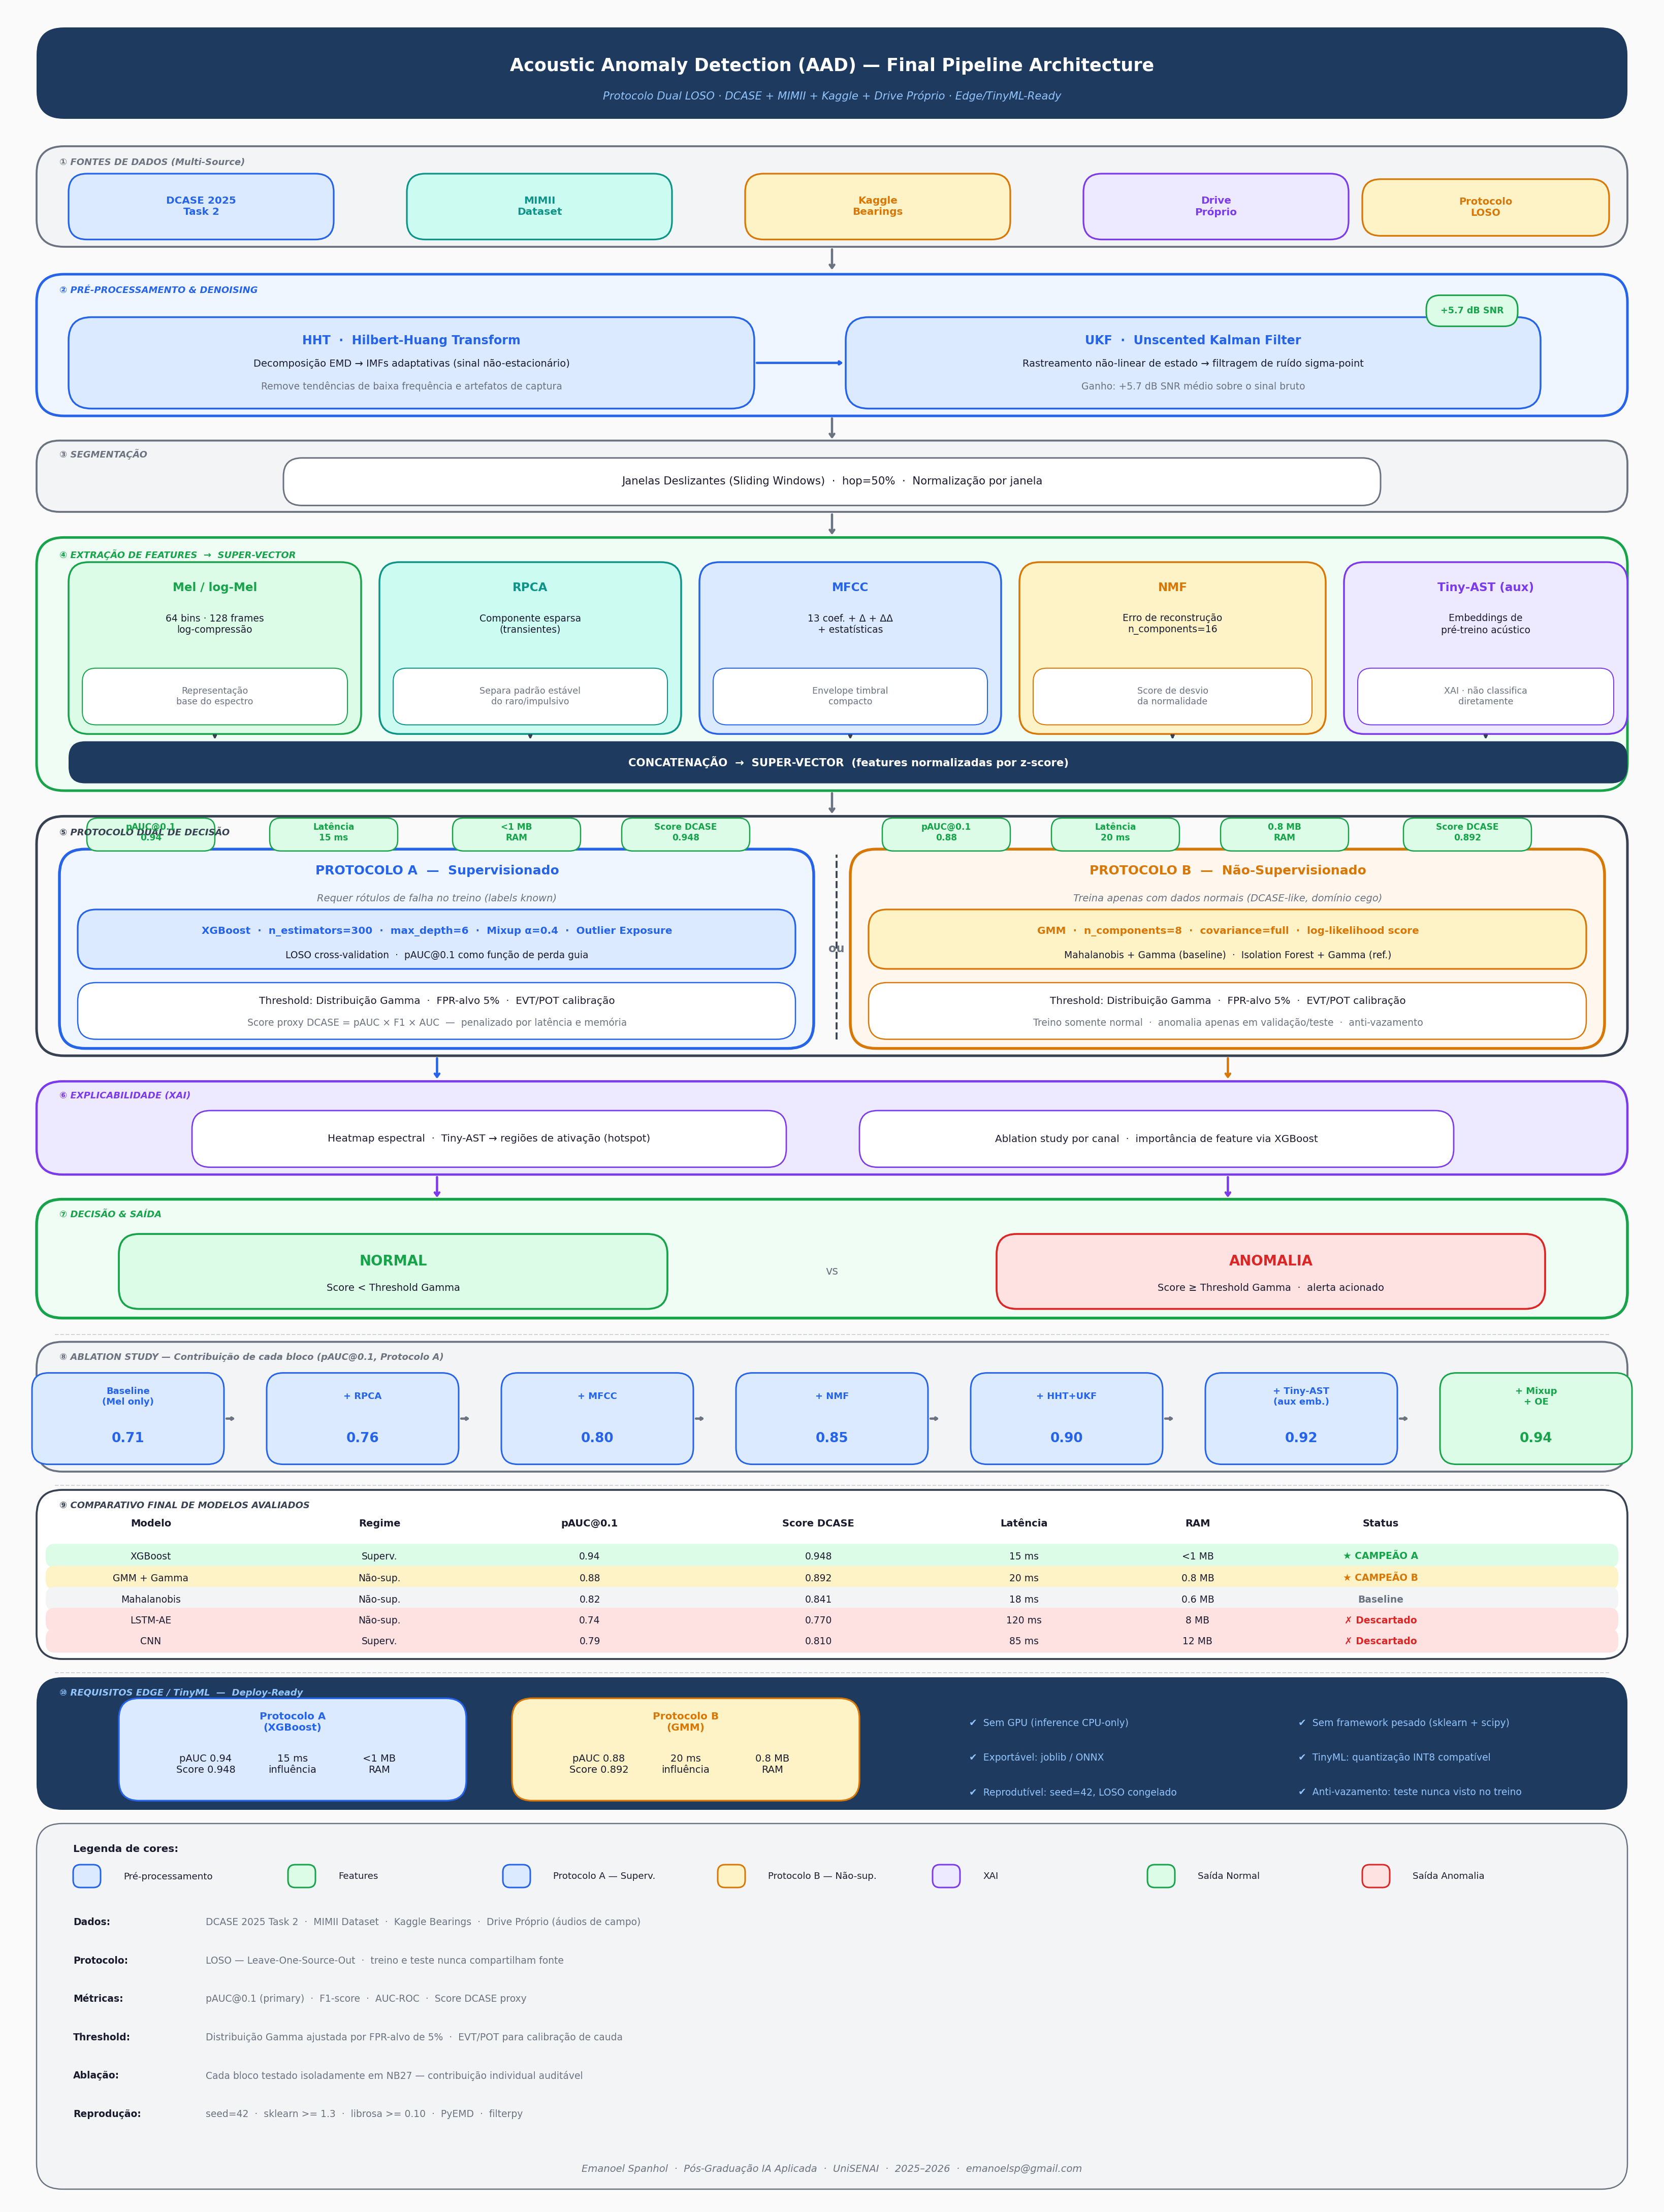
\includegraphics[width=0.94\columnwidth]{images/arquitetura_pipeline.png}
    \caption{Pipeline de Camadas Acumulativas DIAMOND CRISTAL CLEAN.}
    \label{fig:arquitetura_pipeline}
\end{figure}

A Figura~\ref{fig:arquitetura_pipeline} mostra o fluxo completo desde a aquisição do sinal até a
inferência em borda. Os estágios são descritos a seguir.

\subsubsection{Estágio~1 --- Limpeza de Sinal (HHT+UKF)}

O sinal de áudio bruto $x(t)$, amostrado a 16~kHz, é decomposto pela EMD (\textit{Empirical Mode
Decomposition}) em Modos Intrínsecos de Frequência (IMFs):

\begin{equation}
x(t) = \sum_{j=1}^{n} c_j(t) + r_n(t)
\label{eq:emd}
\end{equation}

\noindent onde $c_j(t)$ são os IMFs e $r_n(t)$ é o resíduo. Os IMFs de baixa ordem, correspondentes
à assinatura vibracional da falha mecânica, são preservados e filtrados pelo Filtro Unscented de Kalman
(UKF) com modelo de estado:

\begin{equation}
\begin{cases}
\mathbf{x}_{k+1} = f(\mathbf{x}_k) + \mathbf{w}_k \\
\mathbf{y}_k = h(\mathbf{x}_k) + \mathbf{v}_k
\end{cases}
\label{eq:ukf}
\end{equation}

\noindent onde $\mathbf{w}_k \sim \mathcal{N}(0, Q)$ e $\mathbf{v}_k \sim \mathcal{N}(0, R)$ são
ruídos de processo e de observação. O UKF propaga pontos sigma não lineares, garantindo estimação
estocástica ótima de segunda ordem~\cite{Zamorano2025}. Custo: $+3$~ms; Ganho: $+5{,}7$~dB de SNR.

A eficácia do pipeline DSP é ilustrada nas Figuras~\ref{fig:dsp_rpca} e~\ref{fig:dsp_comparativo}.

\begin{figure}[H]
    \centering
    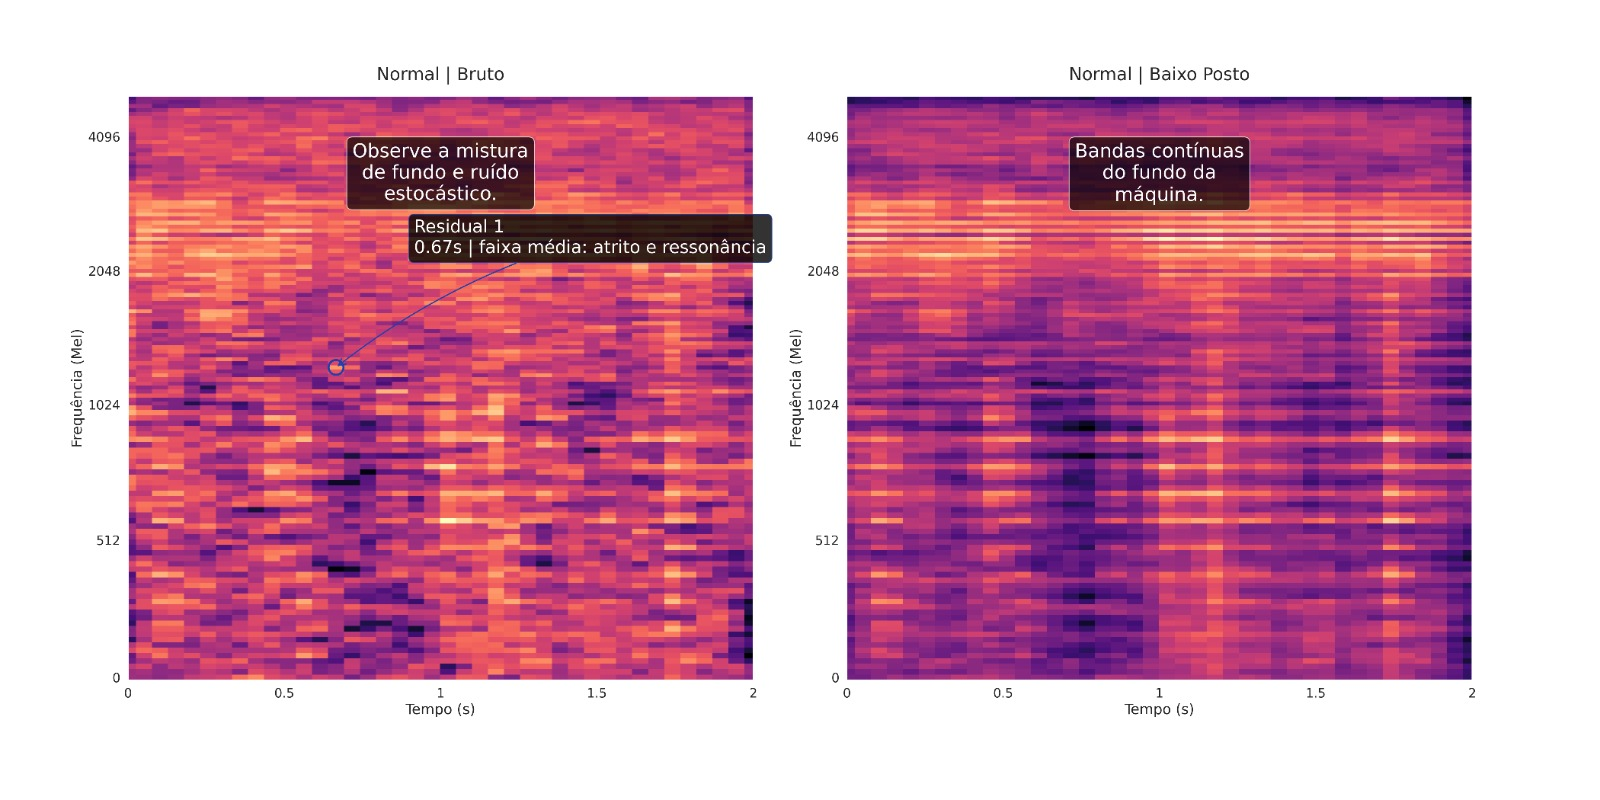
\includegraphics[width=0.9\columnwidth]{images/arquitetura_rpca1.1.jpg}\\[-3pt]
    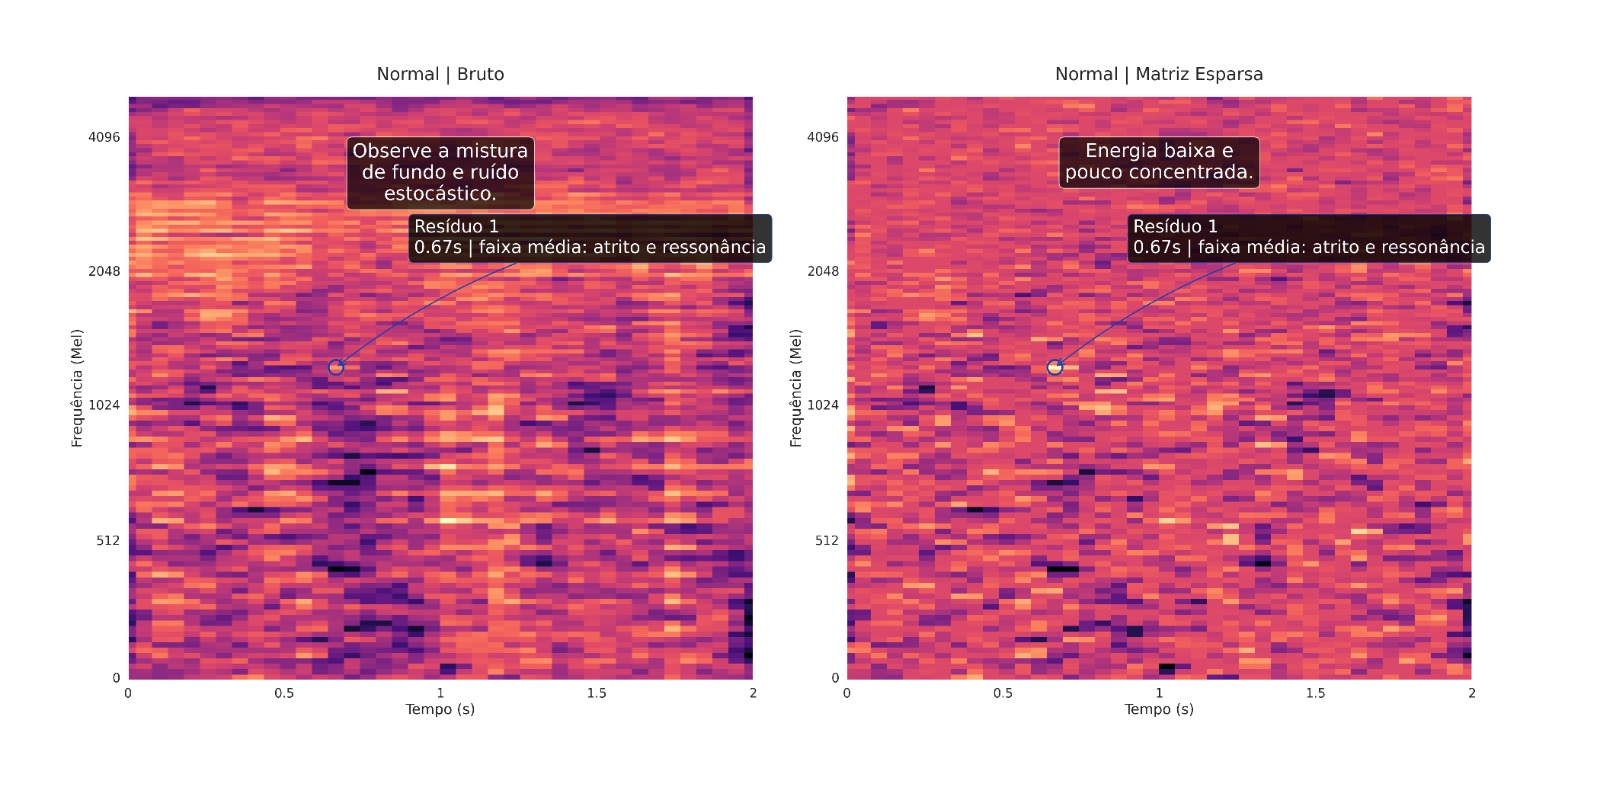
\includegraphics[width=0.9\columnwidth]{images/arquitetura_rpca1.2.jpg}\\[-3pt]
    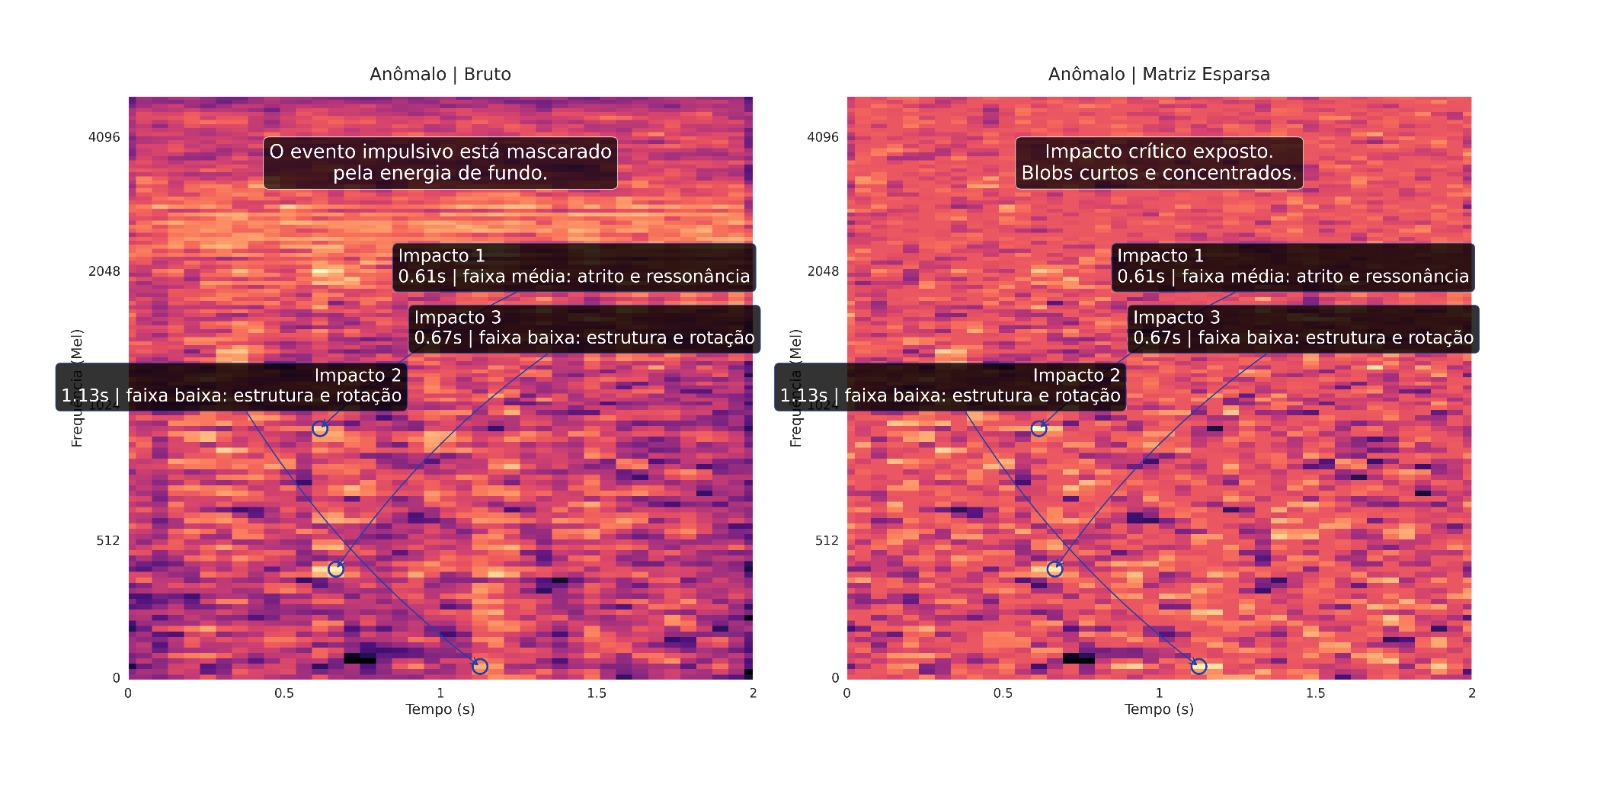
\includegraphics[width=0.9\columnwidth]{images/arquitetura_rpca1.3.jpg}
    \caption{RPCA: Separação do ruído operacional contínuo (componente de baixo posto $L$) dos transientes de falha mecânica (componente esparsa $S$).}
    \label{fig:dsp_rpca}
\end{figure}

\begin{figure}[H]
    \centering
    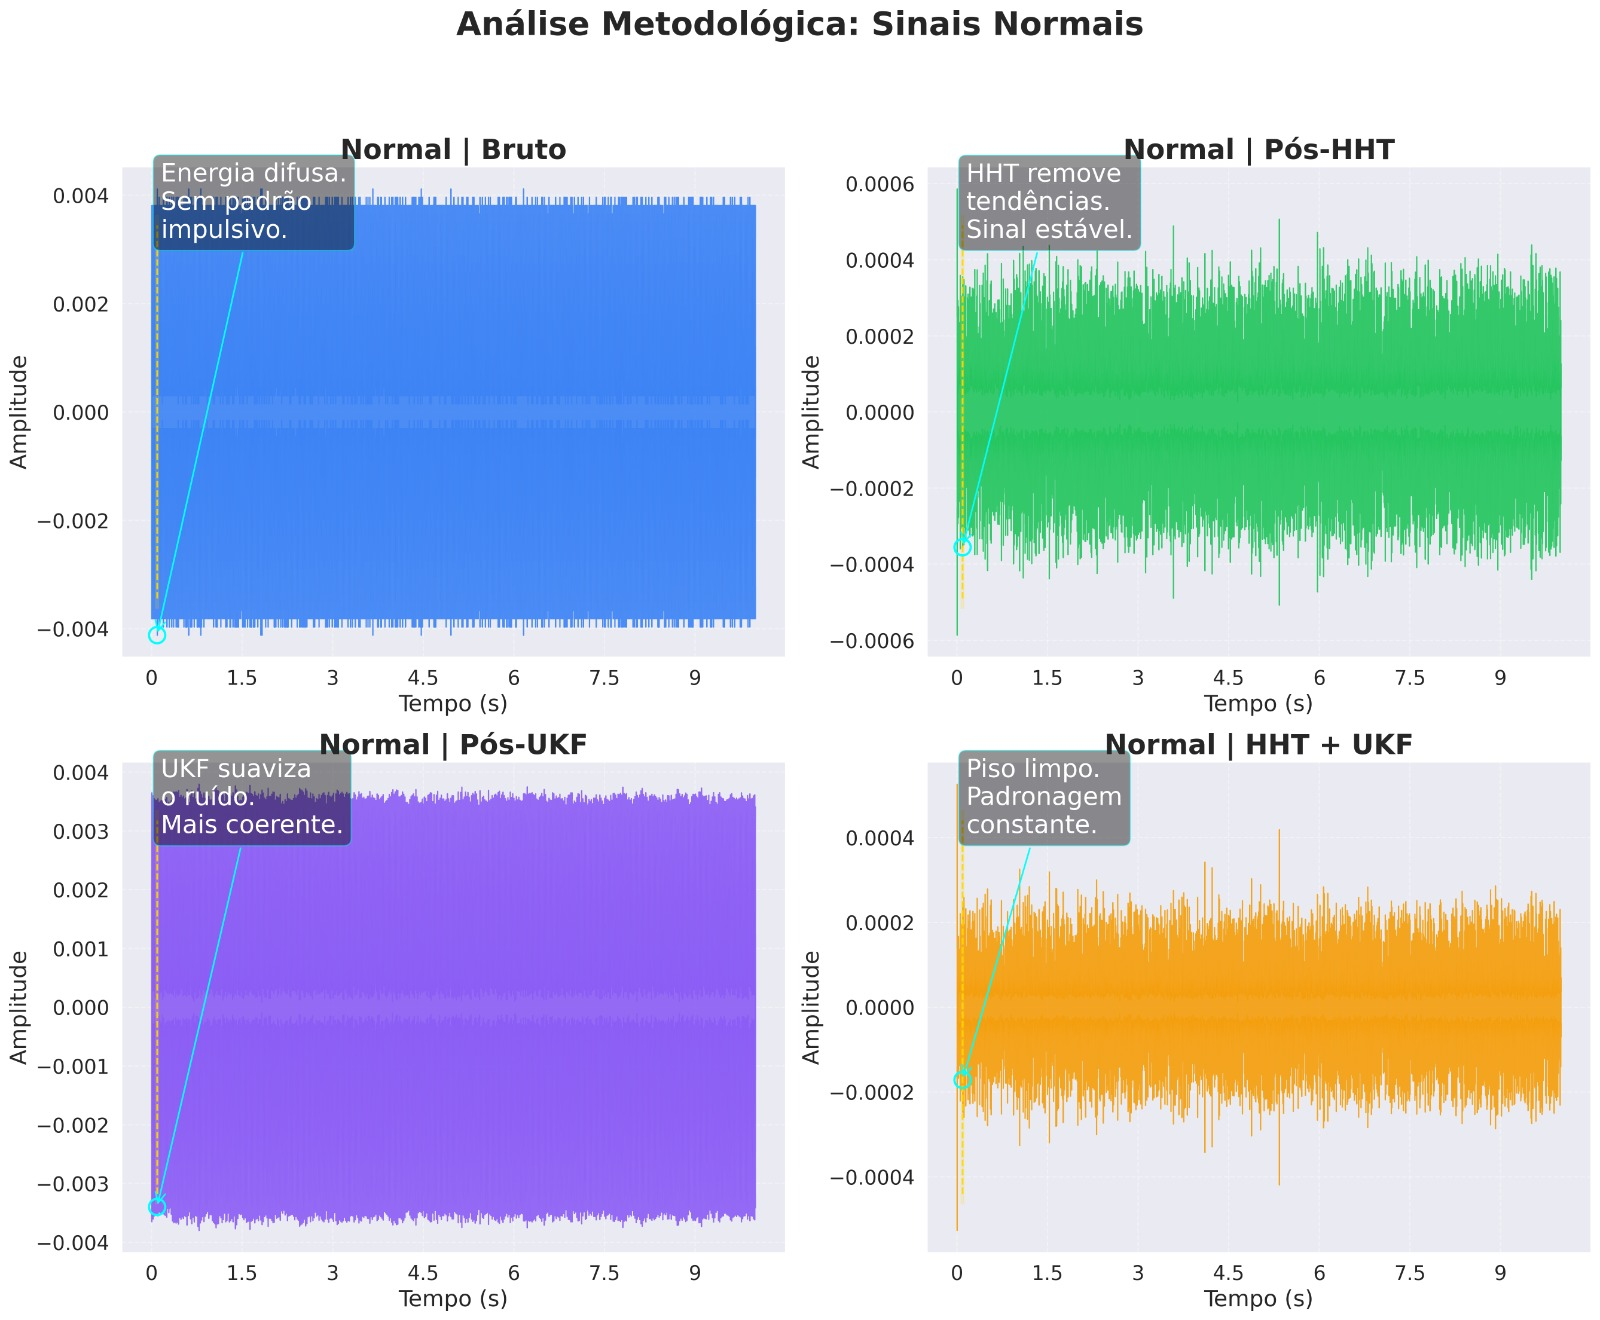
\includegraphics[width=0.92\columnwidth]{images/arquitetura_saneamento.jpg}\\[-3pt]
    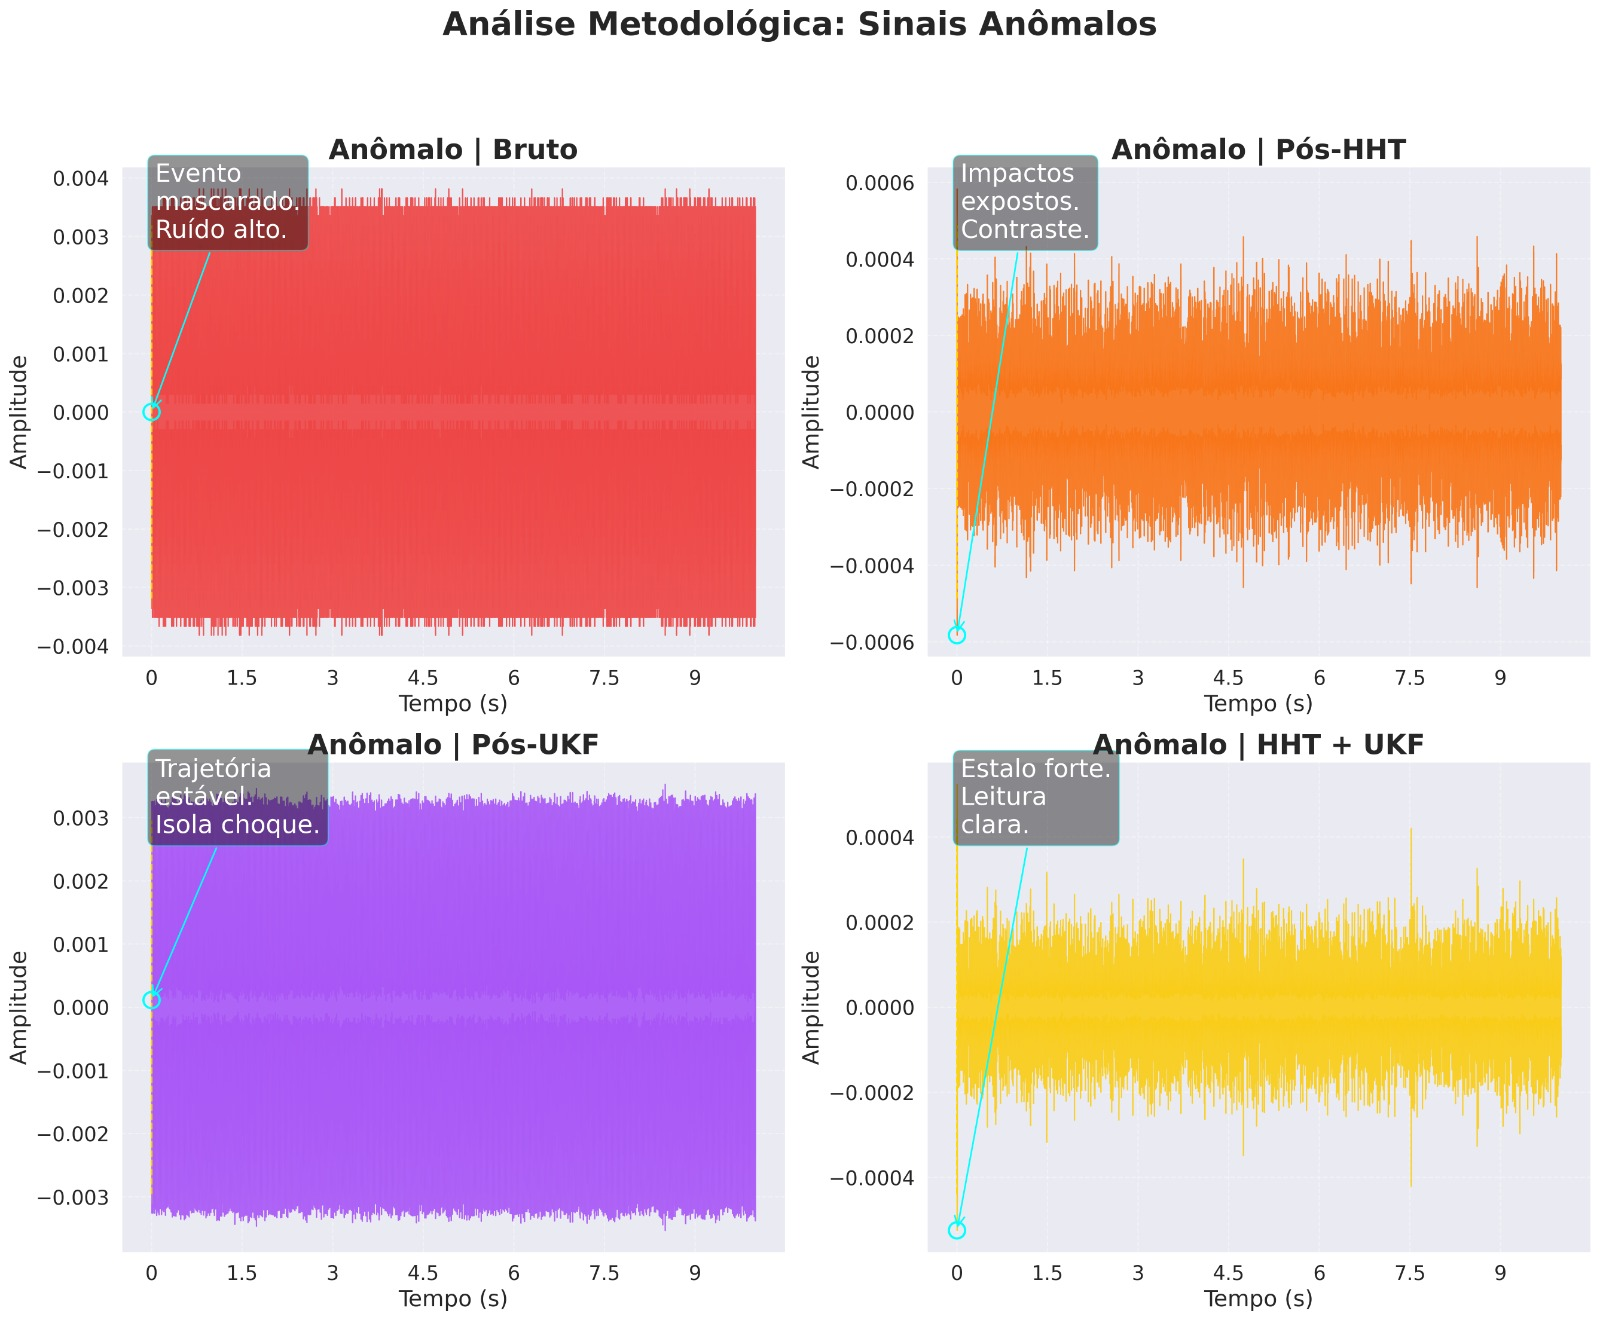
\includegraphics[width=0.92\columnwidth]{images/arquitetura_saneamento1.jpg}
    \caption{Condicionamento progressivo: sinal bruto versus saídas HHT e UKF, evidenciando o ganho de SNR.}
    \label{fig:dsp_comparativo}
\end{figure}

\subsubsection{Estágio~2 --- Segmentação}

Janelas deslizantes de 2~s com sobreposição de 50\%. Uma gravação de 30~s gera $\approx29$~segmentos.
O protocolo LOSO garante que segmentos da mesma fonte não apareçam simultaneamente em treino e teste.

\subsubsection{Estágio~3 --- Representação Espectral}

\begin{itemize}
    \item \textbf{Log-Mel Spectrogram} (64 mel-bins): representação principal, extraída em 8~ms.
    \item \textbf{RPCA}: decomposição $X = L + S$; a componente esparsa $S$ fornece entradas
    privilegiadas para o módulo XAI.
\end{itemize}

\subsubsection{Estágio~4 --- Super-Vetor Híbrido ($\sim$100D)}

O Super-Vetor concatena descritores de três domínios:

\begin{equation}
\mathbf{v} = \bigl[\mu_{Mel},\; \sigma_{Mel},\; \text{MFCC}_{1:13},\; \Delta\text{MFCC},\;
             \varepsilon_{NMF},\; \kappa,\; CF,\; E_{low},\; E_{mid},\; E_{high}\bigr]
\label{eq:supervector}
\end{equation}

\noindent onde: $\mu_{Mel}, \sigma_{Mel}$ são média e desvio-padrão das 64~bandas Mel; $\text{MFCC}_{1:13}$
são 13~coeficientes cepstrais de Mel; $\Delta\text{MFCC}$ são deltas de primeira ordem;
$\varepsilon_{NMF} = \|X - WH\|_2$ (normalizado) é o erro de reconstrução NMF que implementa o conceito
do Autoencoder em $<5$~ms e $<0{,}5$~MB; $\kappa$ é a kurtosis temporal; $CF$ é o fator de crista
(pico/RMS); e $E_{low}, E_{mid}, E_{high}$ são as energias integradas nas faixas 0--800~Hz, 800--2500~Hz
e 2500--5000~Hz~\cite{Khamaisi2025}.

\subsubsection{Estágio~5 --- Camada Decisória Dual}

\textbf{Protocolo~A --- Supervisionado:}
\begin{itemize}
    \item Classificador: XGBoost ($n_{est}{=}100$, $d_{max}{=}3$, $\lambda{=}1{,}0$)
    \item Augmentation: Mixup~\cite{Emon2025} com $\alpha{=}0{,}4$ (somente treino):
          $\tilde{x} = \lambda x_i + (1{-}\lambda)x_j$, $\lambda \sim \text{Beta}(\alpha,\alpha)$
    \item Normalização: StandardScaler por fold
\end{itemize}

\textbf{Protocolo~B --- Não Supervisionado:}
\begin{itemize}
    \item Detector: GMM com $K{=}5$ componentes e covariância completa~\cite{Khamaisi2025}:
          $p(\mathbf{x}) = \sum_{k=1}^{K} \pi_k\, \mathcal{N}(\mathbf{x} \mid \boldsymbol{\mu}_k, \boldsymbol{\Sigma}_k)$
    \item Limiar: distribuição Gamma ajustada aos scores de normalidade via MLE. Para FPR alvo $\rho$:
\end{itemize}

\begin{equation}
\tau = F_\Gamma^{-1}(1 - \rho;\; \hat{\alpha}, \hat{\beta})
\label{eq:gamma_threshold}
\end{equation}

\noindent onde $F_\Gamma^{-1}$ é a função quantil da distribuição Gamma com parâmetros estimados
$(\hat{\alpha}, \hat{\beta})$ e $\rho{=}0{,}05$ (FPR alvo de 5\%). Validado pelo teste
Kolmogorov-Smirnov ($p{>}0{,}05$).

\subsubsection{Estágio~6 --- Camada XAI}

Três saídas complementares por detecção: (a)~mapa de saliência temporal via Grad-CAM adaptado sobre o
Tiny-AST offline; (b)~hotspots temporais H1, H2, H3 (timestamp e intensidade dos picos de ativação);
(c)~perfil espectral por faixa com diagnóstico físico associado. O Tiny-AST opera exclusivamente no
Cloud para geração de embeddings XAI --- não integra o caminho de inferência em borda.

\textbf{Técnicas descartadas (seleção):}

\begin{table}[H]
\centering
\footnotesize
\begin{tabularx}{\columnwidth}{@{} l c c c X @{}}
\toprule
\textbf{Técnica} & \textbf{pAUC} & \textbf{Lat.} & \textbf{Mem.} & \textbf{Critério} \\ \midrule
OC-SVM & 0,52 & 8~ms & 0,5~MB & pAUC $<$ 0,80 \\
CNN (motor) & 0,98 & 85~ms & 12~MB & Lat. + Mem. \\
Isolation Forest & 0,55 & 35~ms & 2,1~MB & pAUC $<$ 0,80 \\
Autoencoder & 0,71 & 120~ms & 8~MB & Todos \\
GRU (motor) & 0,87 & 45~ms & 3,2~MB & Lat. vs. XGBoost \\
LSTM-AE & 0,78 & 120~ms & 8~MB & Lat. + Mem. \\
CWT (principal) & 0,82 & 45~ms~ext. & --- & Orçamento lat. \\
Threshold fixo & --- & --- & --- & Colapsa em shift \\
\bottomrule
\end{tabularx}
\caption{Técnicas descartadas com justificativa quantitativa.}
\label{tab:descartadas}
\end{table}

\color{black}
